% !TeX program = pdflatex
% !TeX root = FCReplaceMomenta.tex

\documentclass[../FeynCalcManual.tex]{subfiles}
\begin{document}
\hypertarget{fcreplacemomenta}{
\section{FCReplaceMomenta}\label{fcreplacemomenta}\index{FCReplaceMomenta}}

\texttt{FCReplaceMomenta[\allowbreak{}exp,\ \allowbreak{}rule]} replaces
the given momentum according to the specified replacement rules. Various
options can be used to customize the replacement procedure.

\subsection{See also}

\hyperlink{toc}{Overview},
\hyperlink{fcpermutemomentarules}{FCPermuteMomentaRules}.

\subsection{Examples}

\begin{Shaded}
\begin{Highlighting}[]
\NormalTok{amp }\ExtensionTok{=}\NormalTok{ (}\SpecialCharTok{{-}}\FunctionTok{I}\NormalTok{)}\SpecialCharTok{*}\NormalTok{Spinor}\OperatorTok{[}\SpecialCharTok{{-}}\NormalTok{Momentum}\OperatorTok{[}\NormalTok{l2}\OperatorTok{],}\NormalTok{ ME}\OperatorTok{,} \DecValTok{1}\OperatorTok{]}\NormalTok{ . GA}\OperatorTok{[}\SpecialCharTok{\textbackslash{}}\OperatorTok{[}\NormalTok{Mu}\OperatorTok{]]}\NormalTok{ . Spinor}\OperatorTok{[}\NormalTok{Momentum}\OperatorTok{[}\NormalTok{l1}\OperatorTok{],}\NormalTok{ ME}\OperatorTok{,} \DecValTok{1}\OperatorTok{]}\SpecialCharTok{*}
\NormalTok{   Spinor}\OperatorTok{[}\NormalTok{Momentum}\OperatorTok{[}\NormalTok{p1}\OperatorTok{],}\NormalTok{ SMP}\OperatorTok{[}\StringTok{"m\_Q"}\OperatorTok{],} \DecValTok{1}\OperatorTok{]}\NormalTok{ . GS}\OperatorTok{[}\NormalTok{Polarization}\OperatorTok{[}\NormalTok{kp}\OperatorTok{,} \SpecialCharTok{{-}}\FunctionTok{I}\OperatorTok{,} 
\NormalTok{      Transversality }\OtherTok{{-}\textgreater{}} \ConstantTok{True}\OperatorTok{]]}\NormalTok{ . (GS}\OperatorTok{[}\NormalTok{kp }\SpecialCharTok{+}\NormalTok{ p1}\OperatorTok{]} \SpecialCharTok{+}\NormalTok{ SMP}\OperatorTok{[}\StringTok{"m\_Q"}\OperatorTok{]}\NormalTok{) . GA}\OperatorTok{[}\SpecialCharTok{\textbackslash{}}\OperatorTok{[}\NormalTok{Mu}\OperatorTok{]]}\NormalTok{ . Spinor}\OperatorTok{[}\SpecialCharTok{{-}}\NormalTok{Momentum}\OperatorTok{[}\NormalTok{p2}\OperatorTok{],} 
\NormalTok{     SMP}\OperatorTok{[}\StringTok{"m\_Q"}\OperatorTok{],} \DecValTok{1}\OperatorTok{]}\SpecialCharTok{*}\NormalTok{FAD}\OperatorTok{[}\NormalTok{kp }\SpecialCharTok{+}\NormalTok{ p1 }\SpecialCharTok{+}\NormalTok{ p2}\OperatorTok{,}\NormalTok{ Dimension }\OtherTok{{-}\textgreater{}} \DecValTok{4}\OperatorTok{]}\SpecialCharTok{*}\NormalTok{FAD}\OperatorTok{[\{}\SpecialCharTok{{-}}\NormalTok{l1 }\SpecialCharTok{{-}}\NormalTok{ l2 }\SpecialCharTok{{-}}\NormalTok{ p2}\OperatorTok{,}\NormalTok{ SMP}\OperatorTok{[}\StringTok{"m\_Q"}\OperatorTok{]\},} 
\NormalTok{    Dimension }\OtherTok{{-}\textgreater{}} \DecValTok{4}\OperatorTok{]}\SpecialCharTok{*}\NormalTok{SDF}\OperatorTok{[}\NormalTok{cq}\OperatorTok{,}\NormalTok{ cqbar}\OperatorTok{]}\SpecialCharTok{*}\NormalTok{SMP}\OperatorTok{[}\StringTok{"e"}\OperatorTok{]}\SpecialCharTok{\^{}}\DecValTok{3}\SpecialCharTok{*}\NormalTok{SMP}\OperatorTok{[}\StringTok{"Q\_u"}\OperatorTok{]}\SpecialCharTok{\^{}}\DecValTok{2}
\end{Highlighting}
\end{Shaded}

\begin{dmath*}\breakingcomma
-\frac{i \;\text{e}^3 Q_u^2 \delta _{\text{cq}\;\text{cqbar}} \left(\varphi (-\overline{\text{l2}},\text{ME})\right).\bar{\gamma }^{\mu }.\left(\varphi (\overline{\text{l1}},\text{ME})\right) \left(\varphi (\overline{\text{p1}},m_Q)\right).\left(\bar{\gamma }\cdot \bar{\varepsilon }^*(\text{kp})\right).\left(\bar{\gamma }\cdot \left(\overline{\text{kp}}+\overline{\text{p1}}\right)+m_Q\right).\bar{\gamma }^{\mu }.\left(\varphi (-\overline{\text{p2}},m_Q)\right)}{(\overline{\text{kp}}+\overline{\text{p1}}+\overline{\text{p2}})^2 \left((-\overline{\text{l1}}-\overline{\text{l2}}-\overline{\text{p2}})^2-m_Q^2\right)}
\end{dmath*}

\begin{Shaded}
\begin{Highlighting}[]
\NormalTok{FCReplaceMomenta}\OperatorTok{[}\NormalTok{amp}\OperatorTok{,} \OperatorTok{\{}\NormalTok{p1 }\OtherTok{{-}\textgreater{}} \FunctionTok{P} \SpecialCharTok{+} \DecValTok{1}\SpecialCharTok{/}\DecValTok{2} \FunctionTok{q}\OperatorTok{,}\NormalTok{ p2 }\OtherTok{{-}\textgreater{}} \FunctionTok{P} \SpecialCharTok{{-}} \DecValTok{1}\SpecialCharTok{/}\DecValTok{2} \FunctionTok{q}\OperatorTok{\}]} 
 
\FunctionTok{ClearAll}\OperatorTok{[}\NormalTok{amp}\OperatorTok{]}
\end{Highlighting}
\end{Shaded}

\begin{dmath*}\breakingcomma
-\frac{i \;\text{e}^3 Q_u^2 \delta _{\text{cq}\;\text{cqbar}} \left(\varphi (-\overline{\text{l2}},\text{ME})\right).\bar{\gamma }^{\mu }.\left(\varphi (\overline{\text{l1}},\text{ME})\right) \left(\varphi (\overline{\text{p1}},m_Q)\right).\left(\bar{\gamma }\cdot \bar{\varepsilon }^*(\text{kp})\right).\left(\bar{\gamma }\cdot \overline{\text{kp}}+\bar{\gamma }\cdot \left(\overline{P}+\frac{\overline{q}}{2}\right)+m_Q\right).\bar{\gamma }^{\mu }.\left(\varphi (-\overline{\text{p2}},m_Q)\right)}{(\overline{\text{kp}}+2 \overline{P})^2 \left((-\overline{\text{l1}}-\overline{\text{l2}}-\overline{P}+\frac{\overline{q}}{2})^2-m_Q^2\right)}
\end{dmath*}

Notice that \texttt{FCReplaceMomenta} is not suitable for expanding in
4-momenta (soft limits etc.) as it does not check for cases where a
particular substitution yields a singularity. For example, the following
code obviously returns a nonsensical result

\begin{Shaded}
\begin{Highlighting}[]
\NormalTok{FCClearScalarProducts}\OperatorTok{[]}\NormalTok{; }
 
\NormalTok{SPD}\OperatorTok{[}\FunctionTok{q}\OperatorTok{]} \ExtensionTok{=} \DecValTok{0}\NormalTok{; }
 
\NormalTok{FCReplaceMomenta}\OperatorTok{[}\NormalTok{FAD}\OperatorTok{[}\FunctionTok{q} \SpecialCharTok{+} \FunctionTok{p}\OperatorTok{],} \OperatorTok{\{}\FunctionTok{p} \OtherTok{{-}\textgreater{}} \DecValTok{0}\OperatorTok{\}]} 
 
\NormalTok{FCClearScalarProducts}\OperatorTok{[]}\NormalTok{;}
\end{Highlighting}
\end{Shaded}

\begin{dmath*}\breakingcomma
\frac{1}{0}
\end{dmath*}

\texttt{FCReplaceMomenta} equally works with \texttt{FCTopology}
objects. There it is actually the preferred way to perform momentum
shifts. Consider e.g.

\begin{Shaded}
\begin{Highlighting}[]
\NormalTok{ex }\ExtensionTok{=}\NormalTok{ FCTopology}\OperatorTok{[}\NormalTok{topo}\OperatorTok{,} \OperatorTok{\{}\NormalTok{SFAD}\OperatorTok{[\{\{}\NormalTok{p1}\OperatorTok{,} \DecValTok{0}\OperatorTok{\},} \OperatorTok{\{}\DecValTok{0}\OperatorTok{,} \DecValTok{1}\OperatorTok{\},} \DecValTok{1}\OperatorTok{\}],}\NormalTok{ SFAD}\OperatorTok{[\{\{}\NormalTok{p2 }\SpecialCharTok{+}\NormalTok{ p3}\OperatorTok{,} \DecValTok{0}\OperatorTok{\},} \OperatorTok{\{}\DecValTok{0}\OperatorTok{,} \DecValTok{1}\OperatorTok{\},} \DecValTok{1}\OperatorTok{\}],} 
\NormalTok{    SFAD}\OperatorTok{[\{\{}\NormalTok{p2 }\SpecialCharTok{{-}} \FunctionTok{Q}\OperatorTok{,} \DecValTok{0}\OperatorTok{\},} \OperatorTok{\{}\DecValTok{0}\OperatorTok{,} \DecValTok{1}\OperatorTok{\},} \DecValTok{1}\OperatorTok{\}],}\NormalTok{ SFAD}\OperatorTok{[\{\{}\NormalTok{p1 }\SpecialCharTok{+}\NormalTok{ p3 }\SpecialCharTok{{-}} \FunctionTok{Q}\OperatorTok{,} \DecValTok{0}\OperatorTok{\},} \OperatorTok{\{}\DecValTok{0}\OperatorTok{,} \DecValTok{1}\OperatorTok{\},} \DecValTok{1}\OperatorTok{\}]\},} \OperatorTok{\{}\NormalTok{p1}\OperatorTok{,}\NormalTok{ p2}\OperatorTok{,}\NormalTok{ p3}\OperatorTok{\},} \OperatorTok{\{}\FunctionTok{Q}\OperatorTok{\},} \OperatorTok{\{\},} \OperatorTok{\{\}]}
\end{Highlighting}
\end{Shaded}

\begin{dmath*}\breakingcomma
\text{FCTopology}\left(\text{topo},\left\{\frac{1}{(\text{p1}^2+i \eta )},\frac{1}{((\text{p2}+\text{p3})^2+i \eta )},\frac{1}{((\text{p2}-Q)^2+i \eta )},\frac{1}{((\text{p1}+\text{p3}-Q)^2+i \eta )}\right\},\{\text{p1},\text{p2},\text{p3}\},\{Q\},\{\},\{\}\right)
\end{dmath*}

where we want to shift \texttt{p_2} to \texttt{p_2 + Q}. Doing so
naively messes us the topology by invalidating the list of loop momenta

\begin{Shaded}
\begin{Highlighting}[]
\NormalTok{ex }\OtherTok{/.}\NormalTok{ p2 }\OtherTok{{-}\textgreater{}}\NormalTok{ p2 }\SpecialCharTok{+} \FunctionTok{Q} 
 
\NormalTok{FCLoopValidTopologyQ}\OperatorTok{[}\SpecialCharTok{\%}\OperatorTok{]}
\end{Highlighting}
\end{Shaded}

\begin{dmath*}\breakingcomma
\text{FCTopology}\left(\text{topo},\left\{\frac{1}{(\text{p1}^2+i \eta )},\frac{1}{((\text{p2}+\text{p3}+Q)^2+i \eta )},\frac{1}{(\text{p2}^2+i \eta )},\frac{1}{((\text{p1}+\text{p3}-Q)^2+i \eta )}\right\},\{\text{p1},\text{p2}+Q,\text{p3}\},\{Q\},\{\},\{\}\right)
\end{dmath*}

\begin{figure}[!ht]
\centering
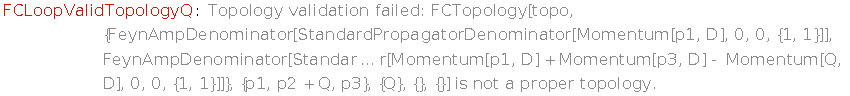
\includegraphics[width=0.6\linewidth]{img/0u1i6qpgdpbjs.pdf}
\end{figure}

\begin{dmath*}\breakingcomma
\text{False}
\end{dmath*}

Using \texttt{FCReplaceMomenta} we immediately get we want

\begin{Shaded}
\begin{Highlighting}[]
\NormalTok{FCReplaceMomenta}\OperatorTok{[}\NormalTok{ex}\OperatorTok{,} \OperatorTok{\{}\NormalTok{p2 }\OtherTok{{-}\textgreater{}}\NormalTok{ p2 }\SpecialCharTok{+} \FunctionTok{Q}\OperatorTok{\}]}
\end{Highlighting}
\end{Shaded}

\begin{dmath*}\breakingcomma
\text{FCTopology}\left(\text{topo},\left\{\frac{1}{(\text{p1}^2+i \eta )},\frac{1}{((\text{p2}+\text{p3}+Q)^2+i \eta )},\frac{1}{(\text{p2}^2+i \eta )},\frac{1}{((\text{p1}+\text{p3}-Q)^2+i \eta )}\right\},\{\text{p1},\text{p2},\text{p3}\},\{Q\},\{\},\{\}\right)
\end{dmath*}
\end{document}
